\newpage
\part{Platforma Gisquick}
\newpage

\section{Úvod do Gisquick}

Gisquick je webová mapová publikační platforma s otevřenými daty. Jejím účelem je snadné a rychlé publikování projektů vytvořených v programu QGIS, které je možné posléze prohlížet webovém rozhraní platformy Quisqick. 
Celá platforma se skládá z několika komponentů (jejich obecné fungování je popsáno v Části I, kapitole 1.2). Komponenty jsou následující.

\subsection{Komponenty}

\begin{itemize}
	\item\textit{Gisquick plugin} - jedná se o zásuvný modul pro program QGIS, pomocí kterého je možné existující projekt publikovat. Použití pluginu je prvním krokem k publikaci předem vytvořeného projektu. Při publikaci si může každý uživatel pomocí pluginu projekt nastavit tak, aby zobrazovaný předmět zájmu přesně odpovídal jeho požadavkům (možnost selekce jednotlivých vrstev, nastavení maximálního a minimálního měřítka, atd.). Gisquick plugin pracuje zcela odděleně od ostatních komponentů a jeho výstupem je složka obsahující všechny použité vrstvy, uložený projekt ve formátu .qgs a metadatový soubor obsahující dodatečné nastavení projektu.
	\item\textit{webový server} - webový server zpracovává dotazy ve formě OGC standardů, které posílá klient a následně odpovídá například ve formě mapových obrázků. Na straně webového serveru je použit framework Django, který je stejně jako Gisquick plugin psaný v jazyce Python.
	\item\textit{QGIS server} - jedná se o webový mapový server na základě kterého jsou vytvářeny mapové obrázky. Použití QGIS serveru je dáno skutečností, že veškeré mapové prvky zde vytvořené korespondují svým vzhledem s těmi vytvořenými v QGIS desktopové aplikaci. Díky tomu si může být uživatel jistý tím, že to co publikuje bude věrně odpovídat jeho původnímu projektu.
	\item\textit{webový a mobilní klient} - klient uživateli nabízí uživatelské rozhraní celé aplikace ve kterém se může orientovat a pomocí kterého interaguje s webovým serverem a tak mění zobrazovaný obsah. Právě této části spolu s Gisquick Pluginem byla je v této práci věnována největší pozornost.
\end{itemize}

\subsection{Uživatelské rozhraní}

\begin{figure}[h!]
	\centering
	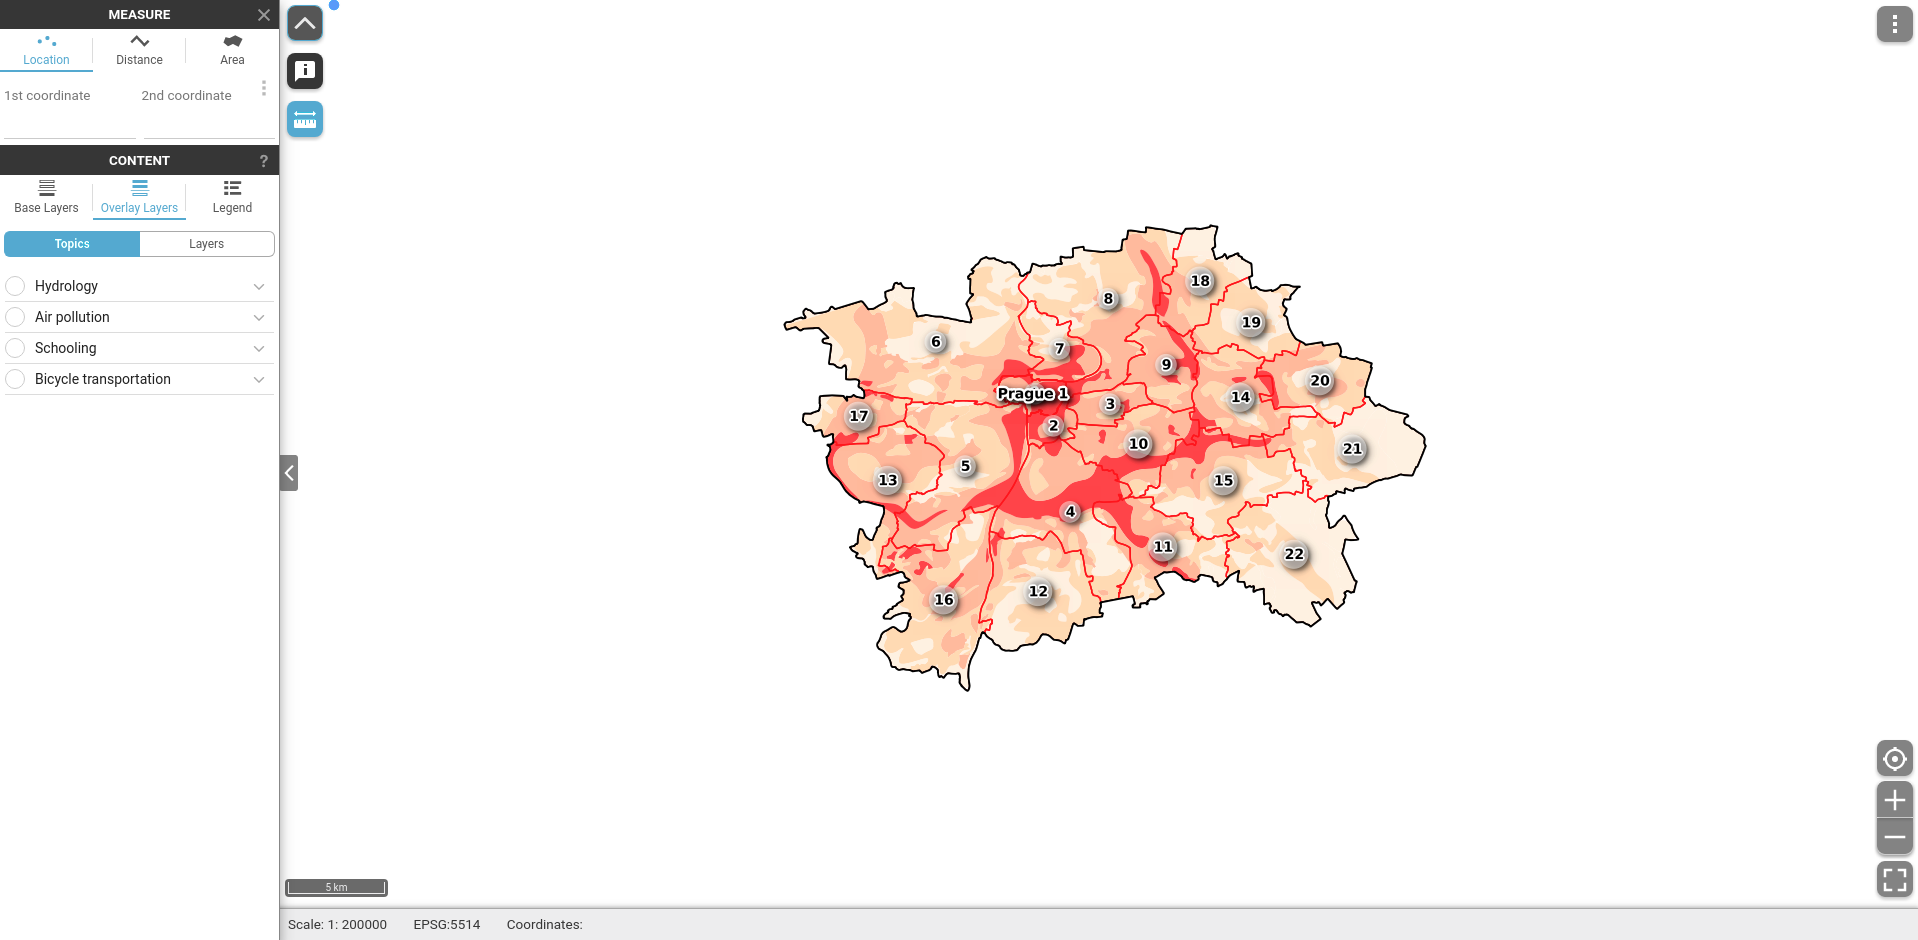
\includegraphics[width=0.9\textwidth]{../img/gisquick_ui.png}
	\caption{screenshot uživatelské rozhraní platformy Gisquick\cite{gisquick-prague}}
	\label{fig:gisquick-prague}
\end{figure}

Obrázek výše zachycuje webové uživatelské rozhraní Gisquick platformy. Jedná se o sadu velice jednoduchých a intuitivních nástrojů sloužících pro snadnou orientaci v publikovaném projektu, filtraci jednotlivých částí a provádění velice jednoduchých operací jako je například měření vzdáleností na mapě.

Uživatel má být schopný rychlé a intuitivní orientace v datech a samotné aplikaci. K tomu slouží postranní menu se správou vrstev spolu s menu nástrojů, které je v přiloženém obrázku rozbaleno. V postranním menu v horní části je právě aktivovaný nástroj sloužící k zjišťování souřadnic, měření vzdáleností a ploch. Hlavní část je věnována samotné interaktivní mapě. Ta poskytuje možnost změny velikosti a polohy zobrazovaného území.

\begin{figure}[h!]
	\centering
	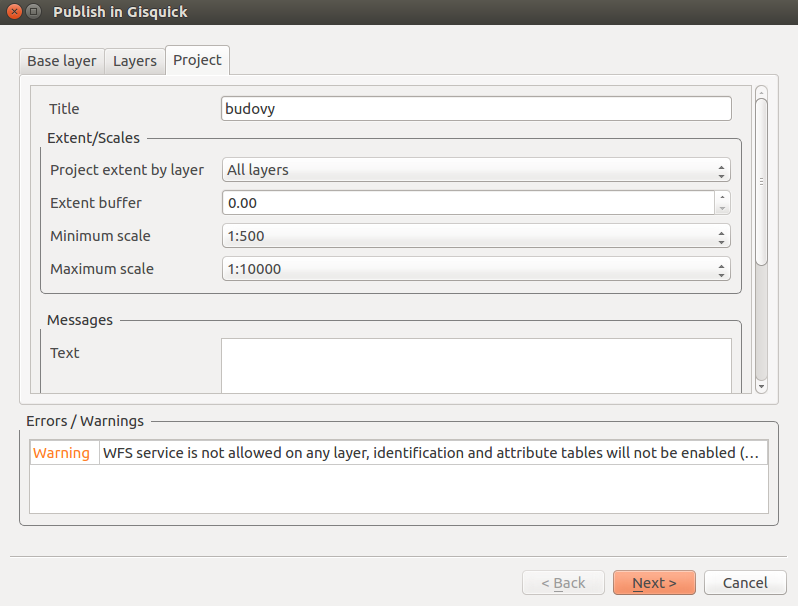
\includegraphics[width=0.7\textwidth]{../img/gisquick_plugin.png}
	\caption{screenshot uživatelské rozhraní Gisquick pluginu pro QGIS}
	\label{fig:gisquick-plugin}
\end{figure}

\newpage
Gisquick plugin rovněž disponuje uživatelským rozhraním, kde pomocí jednoduchého dialogového okna jsou nabízeny možnosti pro export vrstev. Jeho první část je rozdělena na tři záložky a stavovou řádku, kde se jsou vypisovány errory. V první záložce je možno nastavit podkladové vrstvy jako například Open Street Map, nebo Binq mapy. V další záložce je možno nastavit viditelnost jednotlivých vrstev. Při implementaci podpory pro časoprostorová data byly jednotlivé vrstvy rozšířeny o další nastavení. Tomu se bude práce věnovat detailněji v další části. V poslední záložce je obecné nastavení projektu. Další okno slouží k nastavení \textit{topics} nebo-li tématicky orientovaných vrstev \cite{gisquick-manual}. Předposlední stránka obsahuje pouze souhrn publikovaného projektu. A poslední zobrazuje výpis souborů, které se po zmáčknutí tlačítka \textit{Publish} vytvoří. Ty je poté nutné nahrát na Gisquick publikační server.

\newpage
\subsection{Použité technologie}
	
\textbf{Vue.js} - jedná se o moderní framework s otevřeným kódem napsaný v programovacím jazyce JavaScript jehož první verze byla vydaná začátkem roku 2014 Evanem You \cite{vue-history}. Jeho hlavní použití je vývoj uživatelského rozhraní aplikací, tedy na straně klienta. Uživatelské rozhraní je za pomoci Vue.js rozděleno na několik  komponent, kdy každá obsahuje vlastní javascriptové, html a css skripty. Jednotlivé komponenty dělají kód přehlednější a aplikace méně náročnější. Protože vždy jsou použity jenom ty komponenty, které koncový uživatel potřebuje. Mezi další výhody Vue.js patří mimo práce s komponenty jeho reaktivita, možnosti routingu a úpravu objektového modulu dokumentu (DOM).  

Původní verze webového klienta Gisquicku jsou psány za použití frameworku AngularJS. V současné chvíli je však celý klient vytvářen znovu za pomoci medernějšího Vue.js. Z toho důvodu bylo rozšíření platformy o podporu časoprostorových dat na straně klienta psáno ve stejném framevorku Vue.js. Pokud by se nástroj osvědčil pro jeho použití v produkční verzi, nebude nutné do budoucna kód přepisovat.

\bigskip
\noindent
\textbf{Docker} -
 
\bigskip
\noindent
\textbf{PyQt} - 

\newpage
\section{Implementace nástroje pro práci s časoprostorovými daty}

\section{Gisquick plugin pro QGIS}

%\subsection{Mapy a internet}
